\section{问题二：基于共表达图的关键化合物识别}

问题二利用附件二的化合物相关矩阵构建共表达图，结合附件一的化学特征，给出每个感官维度上关联最强的三个化合物。
估计目标 $T_d=(t_{d1},t_{d2},t_{d3})$ 定义为在 250 款啤酒上按控制已选化合物后的秩关联依次最强、且两两不属于同一共表达模块的 3 个化合物。
这是关联定义，不是因果定义。

题目要求找出关键化合物，本章将其操作化为关联结果。
附件中没有干预数据，不能直接推断因果，化学合理性在结果产生后给出机理解释。
唯一独立于这 250 款啤酒的核验是作者发布的加标实验，其结论只在第~\ref{subsec:spike} 节报告。
因此本章的核心是让关联结果可重复、可独立于感官数据检验，而不是宣称因果。

\subsection{基于斯皮尔曼相关的共表达图与平均连接层次聚类}

候选化合物为附件一的 231 列减去 5 个综合指标和 1 个内标，共 225 个。
综合指标 $esters\_sum$、$aroma\_hops\_sum$、$acids\_sum$、$sulfur\_sum$、$kcalperc$ 由其他化合物计算得到，各自几乎是某一个组成成分的副本，与其对应成分的 Spearman 相关系数绝对值分别为 0.92、0.96、0.97、0.78、0.85。
把它们列为候选会使同一信息以总量和成分两次入选，且题目要求的是化合物。
内标 3-甲基-2-丁烯醛在附件八中被标为内标溶液，反映测量过程，不反映啤酒组成。
6 个排除列仍作为图的注释节点保留，用于展示综合指标与成分的关系。

图~\ref{fig:q2-flow} 给出问题二的完整流程。
化合物与感官秩经共表达图、模拟还原支持的图约束前向选择与置换检验，再经日期组重抽和替代方法，得到化学证据与前三项关联候选。

\begin{figure}[htbp]\centering
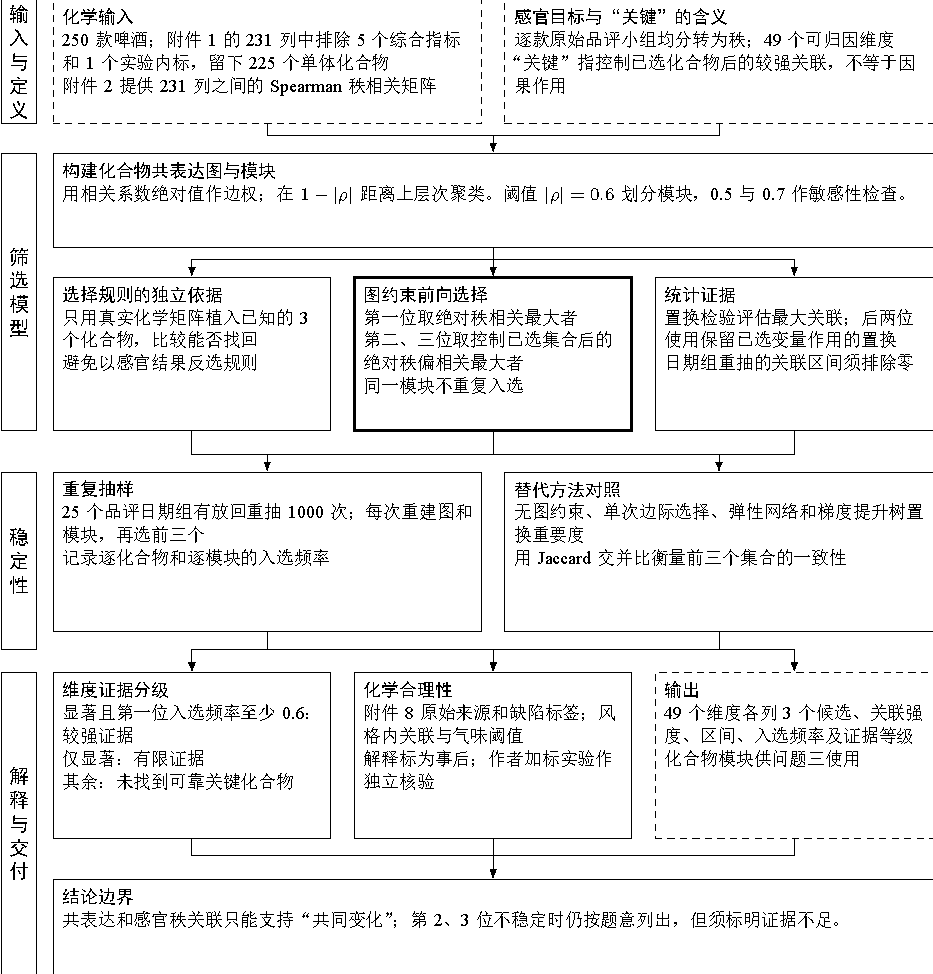
\includegraphics[width=\textwidth]{../figures/q2_methodology_flowchart.pdf}
\caption{问题二方法流程：化合物与感官秩经共表达图、图约束前向选择与置换检验得到关键化合物，稳定性由日期组重抽量化。}
\label{fig:q2-flow}
\end{figure}

共表达图 $G_\tau$ 的节点为 231 列，边权为两两 Spearman 系数的绝对值 $\lvert\rho_{jk}\rvert$，符号作为边属性保留。
使用无符号权重是因为强相关几乎都是正相关，$\lvert\rho\rvert\ge0.5$ 的 597 条边中只有 13 条为负。
模块由 $1-\lvert\rho\rvert$ 上的平均连接层次聚类得到，在高度 $1-\tau$ 处切开。
平均连接只在两组之间平均边权不低于 $\tau$ 时合并，因此每个模块内的化合物彼此平均相关至少约为 $\tau$。

主值 $\tau=0.6$，其依据有三点。
第一，0.6 是候选间 Spearman 相关系数绝对值的 99\% 分位，仅最强的 1\% 化合物对的相关达到该阈值。
第二，$\tau=0.5$ 时模块混入不同来源的化合物，来源纯度（多成员模块中占多数的附件八来源类别所占比例的平均值）降至 0.70，划分可重复性（调整兰德指数 ARI）降至 0.66。
第三，$\tau=0.7$ 时只有 65 个化合物属于多成员模块，冗余控制覆盖的范围变小。
主值下得到 161 个模块，其中 33 个多成员模块覆盖 97 个化合物，代表性模块包括乙醇、乙酸乙酯、己酸乙酯、甘油构成的发酵强度模块，以及辛酸乙酯、癸酸乙酯构成的中链脂肪酸乙酯模块。
化合物层的入选频率在三个 $\tau$ 下相同，所以 $\tau$ 主要影响模块层的解读。

\subsection{共表达模块约束下的秩偏相关前向选择}

第 1 位取边际关联最强者：
\begin{equation}\label{eq:q2-top1}
t_{d1}=\arg\max_{j\in\mathcal C}\,\lvert r_{jd}\rvert .
\end{equation}
其中 $\mathcal C$ 为 225 个候选化合物集合，$r_{jd}$ 是化合物 $j$ 与维度 $d$ 的 Spearman 系数，在两者的标准化秩上计算。
第 $k$ 位（$k=2,3$）在控制已选集合 $S$ 后取秩偏相关最强者。
令 $H_S$ 为向 $\{\mathbf 1,\tilde x_s:s\in S\}$ 张成空间的投影，
\begin{equation}\label{eq:q2-partial}
\begin{aligned}
e_y&=(I-H_S)\tilde y_d,\qquad e_j=(I-H_S)\tilde x_j,\\
r_{jd\mid S}&=\frac{e_j^\top e_y}{\lVert e_j\rVert\,\lVert e_y\rVert},\qquad
t_{dk}=\arg\max_{j\in\mathcal C,\ M(j)\notin M(S)}\,\lvert r_{jd\mid S}\rvert .
\end{aligned}
\end{equation}
式~\eqref{eq:q2-partial} 中 $r_{jd\mid S}$ 是秩上的偏相关，衡量化合物 $j$ 在已选化合物之外还能解释多少维度排序。
图在第一处排除与已选者属于同一模块的化合物，在第二处把同模块化合物与入选者一起报告。

\subsection{模拟实验验证、置换检验与日期组重抽样}

选用前向选择而不用边际选择，由模拟还原实验决定。
边际选择按 $\lvert r_{jd}\rvert$ 降序、每模块至多一个取前 3，会反复选入第 1 个植入化合物的间接相关者。
在真实化学矩阵上随机植入 3 个来自不同模块的化合物，按秩线性组合加噪声生成维度，第 1 个植入化合物的 $r$ 取 0.2、0.3、0.45，权重取 (1, 0.75, 0.5) 与 (1, 1, 1)，每种设置 1,000 次。
前向选择在 $r\ge0.3$ 时找回率更高，其中找回率指植入化合物被选入前 3 位的比例，而观测数据中 49 个维度第 1 位关键化合物的 $\lvert r\rvert$ 中位数为 0.38，四分位为 0.30 到 0.48，处于前向选择占优的区间。
模拟只用化学矩阵，不使用感官数据，因此这一选择没有利用观测到的 Top-3 内容。

图~\ref{fig:q2-recovery} 为 2 乘 3 小多图，行为两种植入权重，列为植入名次 1 到 3。
横轴为第 1 个植入化合物的 $r$，纵轴为化合物层找回率，两条线为前向选择与图约束边际选择。
每格加竖向阴影带，表示 49 维 Top-1 相关绝对值的四分位范围及中位线。
图注写明每格 1,000 次，二项 95\% 区间约正负 0.03，不画误差线。
前向选择在中等与较大效应量下找回率更高，在小效应量下与边际选择相当，两种规则的实际差异按本图呈现。

\begin{figure}[htbp]\centering
\phfig{0.38\textwidth}{2 乘 3 找回率小多图，行为两种权重，列为植入名次 1 到 3，横轴为第 1 个植入化合物的 $r$，纵轴为化合物层找回率。}
\caption{规则依据实验的找回率。两条线为前向选择与图约束边际选择，竖向阴影带为观测 Top-1 相关的四分位范围。}
\label{fig:q2-recovery}
\end{figure}

每个维度的显著性门槛由置换检验给出。
打乱 $\tilde y_d$ 的行 1,000 次，取 225 个化合物边际相关绝对值的最大值，得到维度 $d$ 的零分布，95\% 分位记为 $q_d$。
第 2、3 位用 Freedman--Lane 置换，打乱 $e_y$ 后在可选化合物上取偏相关绝对值的最大值。
逐行打乱忽略日期组内的相关，零分布偏窄，因此每个入选项另外用日期组簇 bootstrap 计算 95\% 置信区间。
入选项同时满足得分超过门槛与置信区间不含 0 时记为显著。

稳定性重抽以日期组为单位，而不是以单款啤酒为单位。
同一天品评的啤酒共享出席名单和品评情境，且大多属于同一风格。
按单款啤酒重抽会把这些相关性当作独立样本，高估有效样本量。
25 个日期组是可直接观测、粒度更粗的分组，重抽时每次抽取 25 个日期组并拼接其中的啤酒。

表~\ref{tab:q2-setup} 按输入与目标、缺失与秩、图与模块、选择规则、显著性、稳定性、规则依据实验、对照方法八个环节列出正文报告的设置。

\begin{table}[htbp]
\centering\small
\caption{问题二实验设置与对照}
\label{tab:q2-setup}
\begin{tabular}{>{\raggedright\arraybackslash}p{3.0cm}>{\raggedright\arraybackslash}p{5.4cm}>{\raggedright\arraybackslash}p{4.2cm}}
\toprule
环节 & 正文报告的设置 & 控制或检验什么 \\
\midrule
输入与目标 & 250 款啤酒；附件一 231 列剔除 5 个综合指标与内标，剩 225 个候选；49 个维度，barnyard 记作同 stale\_hops；感官目标为原始评分均分的秩 & 候选都是化合物或理化指标，目标与问题一同口径 \\
\addlinespace
缺失与秩 & 8 个单化合物列共 60 个空值按列均值填充，每次 bootstrap 样本内重算；信号下限按并列最低秩处理 & 填充值不解释为浓度 \\
\addlinespace
图与模块 & 边权取 $\lvert\rho\rvert$，$1-\lvert\rho\rvert$ 上平均连接层次聚类，$\tau=0.6$ 切割 & 模块内平均相关至少约为 $\tau$ \\
\addlinespace
选择规则 & 第 1 位取最大 $\lvert r_{jd}\rvert$，第 2、3 位取控制已选集合后的秩偏相关最大者，同一模块至多入选 1 个 & 用条件关联去除间接相关者 \\
\addlinespace
显著性 & 置换 1,000 次，第 1 位用全体候选最大相关零分布的 95\% 分位，第 2、3 位用 Freedman--Lane 置换，并同时要求日期组 bootstrap 95\% 置信区间不含 0 & 维度内多重比较与日期组内相关 \\
\addlinespace
稳定性 & 25 个日期组有放回重抽 $B=1000$，每次重建相关矩阵与模块，报告化合物层与模块层入选频率 $\pi^c$、$\pi^m$，分档界限 0.6 与 $1/3$ & 结论对样本扰动的稳定程度 \\
\addlinespace
规则依据实验 & 真实化学矩阵植入 3 个不同模块的化合物，权重 (1,0.75,0.5) 与 (1,1,1)，第 1 个植入化合物的 $r$ 取 0.2、0.3、0.45，每种设置 1,000 次，噪声含日期组偏移 & 只用化学矩阵、不用感官数据，回应根据结果改规则的质疑 \\
\addlinespace
对照方法 & 无图约束边际选择、图约束边际选择、ElasticNet、问题一梯度提升树、风格内分析 & 每种对照对应方法的一处改动 \\
\bottomrule
\end{tabular}
\end{table}

Top-3 是关联而非因果。
维度等级按 Top-1 的显著性与入选频率分为三档，A 级为 Top-1 显著且 $\pi^c\ge0.6$，B 级为 Top-1 显著但不满足 A，C 级为 Top-1 不显著。
选择规则在预运行后由边际选择改为前向选择，已在正文披露。

\subsection{各感官维度的前三项关键化合物与稳定性结果}

\subsubsection{前三项结果与关联方向}

表~\ref{tab:q2-rep} 给出代表维度的 Top-3 证据。
代表维度按事先规则选取，每个维度组至少一个，优先与加标属性对应的维度，含一个 C 级维度，共 21 行。
化学解释写在正文，不入表。
选择得分、95\% 置信区间与风格内系数从最终合理性表导出，完整 147 项按六个维度组放附录。

\begin{table}[htbp]
\centering\small
\caption{代表维度的 Top-3 证据}
\label{tab:q2-rep}
\begin{tabular}{lclclcl}
\toprule
维度（等级） & 名次 & 化合物 & 方向 & $\pi^c$ & OAV$\ge$1 占比 \\
\midrule
A\_esters\_all（A） & 1 & 己醇 & $+$ & 0.61 & 无阈值 \\
 & 2 & 乳酸 & $+$ & 0.36 & 0.17 \\
 & 3 & 乙醛 & $+$ & 0.33 & 0.00 \\
\addlinespace
F\_malt\_all（A） & 1 & pH & $+$ & 0.79 & 无阈值 \\
 & 2 & 乙醇 & $+$ & 0.47 & 0.98 \\
 & 3 & 色度 & $+$ & 0.47 & 无阈值 \\
\addlinespace
bitternes（A） & 1 & 苦味单位 & $+$ & 1.00 & 0.86 \\
 & 2 & 辛酸乙酯 & $+$ & 0.74 & 0.26 \\
 & 3 & 铁 & $-$ & 0.09 & 0.48 \\
\addlinespace
body（A） & 1 & 乙醇 & $+$ & 0.99 & 0.98 \\
 & 2 & 色度 & $+$ & 0.56 & 无阈值 \\
 & 3 & 铁 & $-$ & 0.04 & 0.48 \\
\addlinespace
lactic（A） & 1 & pH & $-$ & 0.95 & 无阈值 \\
 & 2 & 乙酸异戊酯 & $-$ & 0.88 & 0.84 \\
 & 3 & 蛋白质 & $+$ & 0.53 & 1.00 \\
\addlinespace
clove（A） & 1 & 柠檬烯 & $+$ & 0.80 & 无阈值 \\
 & 2 & $\alpha$-卡拉烯 & $-$ & 0.21 & 无阈值 \\
 & 3 & 乙酸丙酯 & $+$ & 0.20 & 无阈值 \\
\addlinespace
t2n（C） & 1 & $\beta$-水芹烯 & $-$ & 0.23 & 无阈值 \\
 & 2 & 辛酸乙烯酯 & $+$ & 0.18 & 无阈值 \\
 & 3 & 己醇 & $-$ & 0.04 & 无阈值 \\
\bottomrule
\end{tabular}
\end{table}

\subsubsection{化合物及模块入选频率}

图~\ref{fig:q2-network} 重绘共表达网络，只画多成员模块的化合物和 6 个注释节点，单成员节点只在图注计数。
节点颜色为附件八来源，大小为该化合物进入主方法 Top-3 的维度数，未入选者空心。
边宽与 $\lvert\rho\rvert$ 成正比，负相关边虚线。
标注至少 3 个成员模块的枢纽、全部入选化合物，以及发酵强度、中链脂肪酸乙酯等代表模块。

\begin{figure}[htbp]\centering
\phfig{0.40\textwidth}{共表达网络，节点按附件八来源着色、按入选维度数定大小，模块内力导向排布，边宽与相关绝对值成正比。}
\caption{化合物共表达网络。只画多成员模块与注释节点，图注计数单成员节点并说明综合指标的排除理由。}
\label{fig:q2-network}
\end{figure}

图~\ref{fig:q2-stability} 左栏为 49 行乘 3 名次的化合物层入选频率 $\pi^c$ 热图，行按六个维度组分块，三档离散色阶，格内写两位小数，不显著项加斜线纹。
右栏为名次 1 到 3 各一根堆叠柱，按稳定、中等、不稳定的维度数堆叠，叠加化合物层与模块层入选频率的均值标记，两者之差反映同模块轮换。
入选频率按名次为 0.60、0.36、0.22，稳定、中等、不稳定项分别为 33、41、73。
此图支持多数维度可靠支持的关键化合物为 1 到 2 个这一结论。

\begin{figure}[htbp]\centering
\phfig{0.44\textwidth}{左栏为 49 行乘 3 名次的入选频率热图，行按六个维度组分块；右栏为三个名次各一根堆叠柱。}
\caption{关键化合物的稳定性。左栏为逐维入选频率热图，右栏为三个名次按稳定程度堆叠的维度数。}
\label{fig:q2-stability}
\end{figure}

\subsubsection{证据分级与支持不足的维度}

图~\ref{fig:q2-jaccard} 为竖向柱状图，横轴为五个方法，纵轴为 49 维平均 Jaccard，每个方法画化合物层、模块层两根柱，柱顶标 Top-1 一致比例。
Jaccard 系数为两个集合交集与并集大小之比，衡量两个方法选出化合物的重合程度。
随机 3 元集合基线 0.008 画细虚线，说明重合不是偶然。
主方法与无图约束边际选择、图约束边际选择的化合物层 Jaccard 分别为 0.339 与 0.382，Top-1 按构造相同。
与 ElasticNet 为 0.573，与梯度提升树为 0.267，与风格内分析为 0.259。
梯度提升树的 Top-1 一致比例只有 0.45，解释为估计对象不同，相关特征下置换重要度被稀释，不同的维度在附录并列给出。

\begin{figure}[htbp]\centering
\phfig{0.29\textwidth}{方法间 Jaccard 柱状图，横轴为五个方法，纵轴为 49 维平均 Jaccard，每个方法画化合物层、模块层两根柱。}
\caption{方法间 Jaccard。细虚线为随机 3 元集合基线，柱顶标注 Top-1 一致比例。}
\label{fig:q2-jaccard}
\end{figure}

显著性门槛 $q_d$ 的中位数为 0.229，第 1、2、3 位超过门槛的维度分别为 48、39、21 个。
维度等级为 A 级 26 个、B 级 22 个、C 级 1 个，C 级为 t2n。
共变标记项数 88 个，模块不可分假设被推翻 0 项。
附件二与附件六的复算误差分别为 $2.05\times10^{-15}$ 与 $6.66\times10^{-16}$，说明列对齐与逐对删除的实现正确。
C 级维度 t2n 的零膨胀检查未发现关联随零膨胀而增强的证据。

\subsection{来源标签、气味活度值与混合物加标的化学合理性论证}

\subsubsection{来源、缺陷标签与气味活度值证据}

以苦味为例，苦味单位的入选频率为 1.00，与苦味的关联方向为正，气味活度值超过 1 的啤酒占 86\%。
以乳酸为例，pH 与乳酸感的关联方向为负，说明酸度由 pH 直接刻画。
以 t2n 为例，其 Top-1 不显著，标记为未找到可靠的关键化合物，Top-3 仍列出供参考。

\subsubsection{风格内关联与共变化合物解释}

图~\ref{fig:q2-scatter} 为 147 个点的散点图，横轴为合并边际 Spearman $r_{jd}$，纵轴为风格内 $r^{(s)}_{jd}$，点形状表示名次，颜色表示风格内置信区间是否含 0。
主 Top-3 的 147 项中 98\% 在风格内保持同号，风格内与合并系数之比的中位数为 0.66。
有 18 项的风格内 $\lvert r^{(s)}\rvert<0.1$，即其关联几乎完全来自风格之间，包括乳酸到乳酸感、pH 到酸感、乙醇到麦芽风味。

\begin{figure}[htbp]\centering
\phfig{0.38\textwidth}{合并边际相关对风格内相关的散点，147 个点，标出乳酸到乳酸感、pH 到酸感、乙醇到麦芽风味。}
\caption{合并与风格内关联。参考线为 $y=x$ 与 $y=0$，颜色表示风格内置信区间是否含 0。}
\label{fig:q2-scatter}
\end{figure}

\subsubsection{独立混合物加标实验的对应与解释}
\label{subsec:spike}

表~\ref{tab:q2-spike} 为作者加标实验的同人配对差，加标物为 6 到 7 种化合物的混合物。
酯类加标在三组中都提高 Esters，支持酯类作为酯类维度的关键因素。
未加入任何酒花化合物，Hops 与 Bitterness 不变，是一组阴性对照。
Fullness 在三组中都提高，与 body 的 Top-1 乙醇及其同模块的甘油方向一致，但无乙醇组同样提高，说明甘油或其他成分足以产生该效应。

\begin{table}[htbp]
\centering\small
\caption{加标实验的同人配对差与对应维度}
\label{tab:q2-spike}
\resizebox{0.9\textwidth}{!}{\begin{tabular}{lcccl}
\toprule
属性 & Blond 含乙醇 $n{=}20$ & Blond 无乙醇 $n{=}13$ & NABLAB 无乙醇 $n{=}13$ & 对应维度（Top-1） \\
\midrule
Esters & 0.90（4.7） & 1.08（2.9） & 1.31（5.0） & 酯类（己醇 / 蛋白质） \\
Fullness & 1.30（6.3） & 1.31（3.0） & 1.38（4.8） & body（乙醇） \\
Alcohol warming & 1.10（4.2） & 0.92（4.4） & 0.08（0.6） & alcohol（乙醇） \\
Sweetness & 1.15（4.4） & 0.69（2.0） & 1.00（3.1） & sweetness（癸酸乙酯） \\
Hops & $-0.15$（$-0.5$） & 0.00（0.0） & $-0.08$（$-0.2$） & 酒花（辛酸乙酯 / 苦味单位） \\
Bitterness & 0.05（0.2） & $-0.15$（$-0.6$） & $-0.31$（$-0.9$） & bitternes（苦味单位） \\
Malt & 0.45（2.0） & $-0.23$（$-1.0$） & 0.00（0.0） & 麦芽（色度 / pH） \\
Overall & 1.05（2.8） & 1.15（3.6） & 1.08（3.5） & overall（乙酸乙酯） \\
\bottomrule
\end{tabular}}
\end{table}

\subsection{模块阈值、候选集合与感官目标的敏感性分析}

敏感性分析的主要结论是结论对模块阈值、候选集合、缺失处理与附件取值稳定，唯一的例外是感官目标改用附件四的标准化值后 Top-3 与等级变化较大，结论以原始评分均值为准。
